\section{Vacuum field and Casimir Force}\label{sec:vacuum-and-casimir}

\calloutinfo{%
The vacuum field is present everywhere, even in complete absence of matter or real radiation, and it can produce observable effects. A famous manifestation is the attractive \textbf{Casimir force} between two conducting plates placed in vacuum. The physical origin of the effect is the modification of the vacuum mode structure by the cavity boundaries.
}

We suppose that:
\begin{enumerate}
    \item Outside the cavity, the vacuum energy is that of free space, with a continuous spectrum of modes.
    \begin{equation}\label{eqn:12-continuous-free-space-energy}
    E_\text{free} = \frac{\pi \hbar c}{L} \, \int_0^{\infty} m \, dm 
    \end{equation}
    
    \item Inside the cavity, the boundary conditions discretize the allowed modes, so that the vacuum energy becomes a sum over standing-wave modes.
    \begin{equation}\label{eqn:12-discrete-cavity-energy}
        E_\text{cavity} = \sum_m \hbar \omega_m = \frac{\pi\hbar c}{L} \sum_m m
    \end{equation}
    where we remembered that the mode frequencies are given by $\omega_m = m \pi c / L$ (Eqn.~\ref{eqn:11-single-mode-electric-field}).
\end{enumerate}

Since both contributions are divergent separately, only their difference is physically meaningful after regularization. For two perfectly conducting parallel plates separated by a distance $L$, we can calculate:
\[
\Delta E= E_\text{cavity}-E_\text{free} = 
\frac{\pi \hbar c}{L}\, 
\left(\sum_mm-\int m \, dm  \right) = 
 -\frac{\pi\hbar c}{12}\, \frac{1}{L}
\]

\hl{The energy decreases with the length $L$ of the cavity which means we have a \textbf{pulling force}:}
\begin{equation}\label{eqn:12-casimir-force}
    F = -\frac{\partial\Delta E}{\partial L} = -\frac{\pi \hbar c}{12}\frac{1}{L^2}
\end{equation}

If we consider all the possible polarizations:
\begin{equation}\label{eqn:12-casimir-pressure}
    P = \frac{F}{A} = -\frac{\pi^2\hbar c}{240 L^2}
\end{equation}

The negative sign shows that the force is attractive. Notice that this effect vanishes in the classical limit $\hbar\to 0$, which confirms that it is purely quantum in origin. For a separation of $L=\qty{1}{\micro\meter}$, one finds a very small pressure, of the order of
\begin{equation}\label{eqn:12-casimir-pressure-typical}
P\sim 10^{-3}\,\unit{\newton\per\meter\squared},
\end{equation}

so for an area $A=\qty{1}{\centi\meter\squared}$ the force is of order
\begin{equation}\label{eqn:12-casimir-force-typical}
F\sim 10^{-7}\,\unit{\newton}.
\end{equation}

\begin{figure}[H]
    \centering
    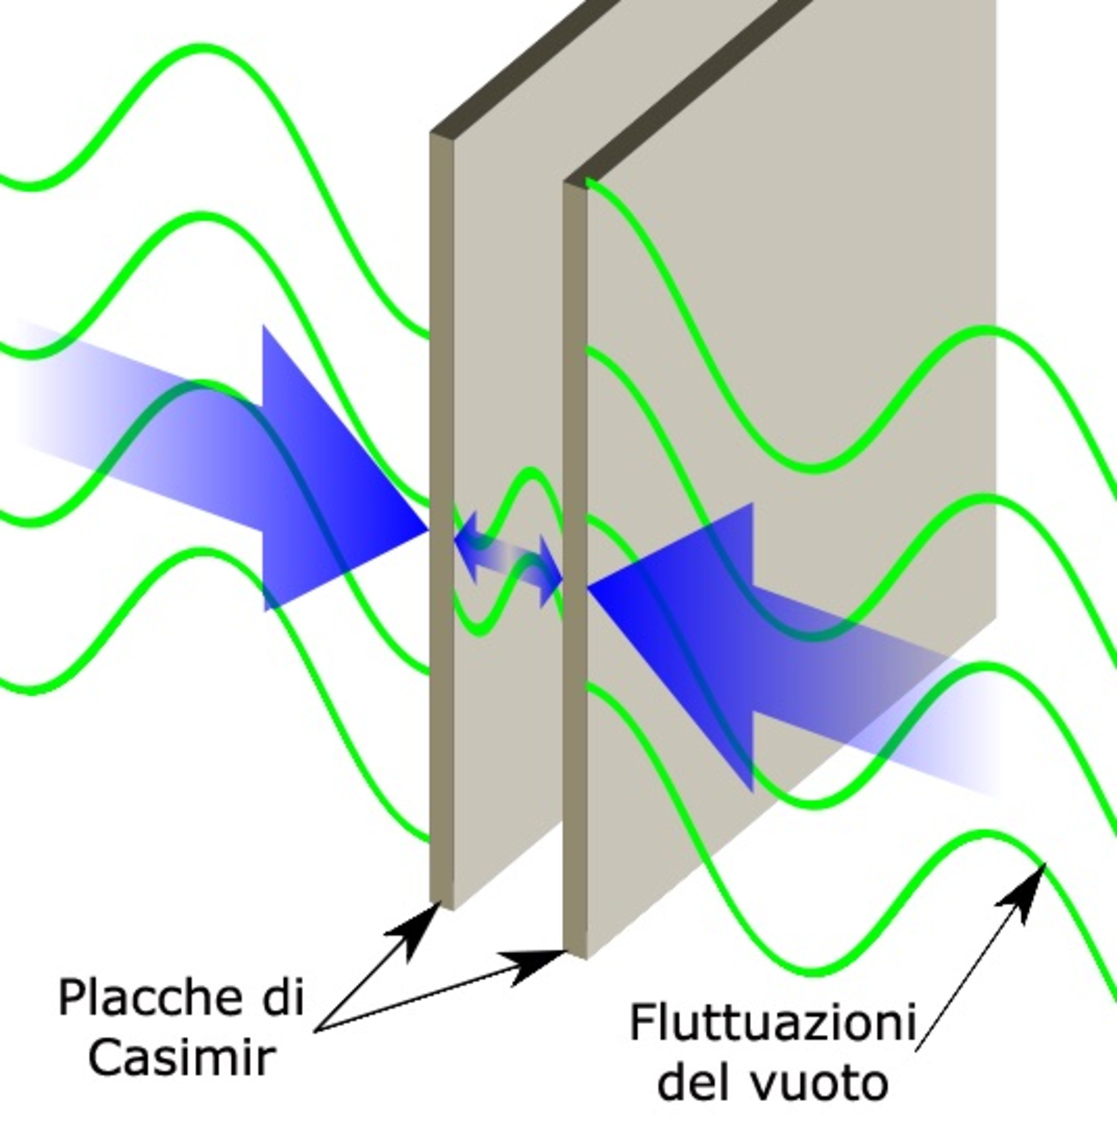
\includegraphics[width=0.4\linewidth]{images_in_pdf/12-/Effetto_Casimir.pdf}
    \caption{Schematic representation of the Casimir effect.}
\end{figure}

\calloutwarn{%
In a real lab, putting two flat plates perfectly parallel at a distance of only $1\,\mu\mathrm{m}$ without letting them touch is practically impossible. If the plates are even slightly tilted, the edges will bump into each other, short-circuiting the setup and ruining the measurement.
}

To solve this practical nightmare, experimentalists use a \textbf{sphere next to a flat plate}. 
This is done because a sphere and a plane always have exactly one single closest point, no matter how you rotate or tilt them; the alignment problem gets removed. The force is then calculated using a standard geometrical correction called the Proximity Force Approximation (PFA).

\subsubsection{Photon localizability}

Observe that photons arise as quantum excitations of the electromagnetic field, but they are also particle-like entities. This raises an important conceptual issue.

\begin{itemize}
    \item \textbf{Classical particles:} a state is fully described by instantaneous position and momentum.
    \item \textbf{Non-relativistic quantum particles:} the operators $\hat{x}$ and $\hat{p}$ do not commute, and the state is described by a wavefunction $\psi(\vec{x})=\langle \vec{x}|\psi\rangle$, which gives the probability amplitude for a position measurement.
    \item For a photon, however, the situation is different: because it is a massless spin-1 particle with gauge constraints and transversality conditions, \hl{there is no fully satisfactory position operator with all the usual properties expected for a localized particle}.
\end{itemize}
    The properties one would like for a photon position operator are:
\begin{itemize}
    \item $[\hat{x},\hat{y}]=0$;
    \item $\hat{x}$ should transform as a vector under rotations.
\end{itemize}

\calloutwarn{%
In practice, these requirements cannot be satisfied simultaneously for the photon in the same way as for massive particles. Therefore, one cannot construct a true position-space wavefunction for the photon in the usual Schrödinger sense.
    
In classical theory, Maxwell equations do not contain any particle concept. In quantum theory, photons are the quanta of the electromagnetic field and  relativistic particles by virtue of their vanishing mass, the correct description requires quantum electrodynamics rather than a single-particle Schrödinger equation.
}